\chapter{Cadre général du projet}
\begin{spacing}{1.2}
\minitoc % Affiche la minitoc du chapitre
\thispagestyle{MyStyle}
\end{spacing}
\clearpage

\section{Introduction}
Ce premier chapitre vise à présenter le projet dans son cadre général en exposant
son contexte, sa problématique ainsi que les objectifs visés. Nous commençons par
présenter l'organisme d'accueil, ses domaines d'expertise et son environnement
technologique. Nous détaillons ensuite le contexte du projet, les limites des
approches existantes et la solution proposée pour répondre aux problématiques
identifiées. Enfin, nous présentons la méthodologie de développement adoptée pour la
réalisation de cette plateforme intelligente orientée Cloud, DevSecOps et
Intelligence Artificielle.

\section{Présentation de l'organisme d'accueil}

\begin{figure}[H]
    \centering
    
\includegraphics[width=0.35\textwidth]{images/Logo_Talan.png}
    \caption{Logo de Talan}
    \label{fig:logo-talan}
\end{figure}

Talan est un groupe international spécialisé dans le conseil en innovation, la
transformation digitale et les technologies avancées. Présent dans plusieurs pays,
le groupe accompagne ses clients dans la modernisation de leurs systèmes
d'information à travers des solutions innovantes intégrant le Cloud Computing, la
Data, l'Intelligence Artificielle et les pratiques DevOps. Grâce à une expertise
multidisciplinaire, l'entreprise participe à la réalisation de projets à forte
valeur technologique destinés à des clients nationaux et internationaux.

\subsection{Services et domaines d'expertise}
Talan Tunisie Consulting intervient dans plusieurs domaines technologiques tels que
le développement logiciel, l'architecture cloud, la cybersécurité, le Data
Engineering, l'Intelligence Artificielle et les pratiques DevSecOps. L'entreprise
propose également des services de transformation digitale, d'intégration de
solutions métiers et d'accompagnement dans l'automatisation des infrastructures
informatiques. Forte de son expertise dans les technologies modernes telles que le
Cloud Computing, Kubernetes, Terraform et les architectures distribuées, elle
contribue à la mise en place de solutions robustes, sécurisées et évolutives,
adaptées aux besoins des organisations.

\subsection{Clients et partenariats stratégiques}
Talan collabore avec de nombreuses entreprises et organisations opérant dans des
secteurs variés tels que la finance, les télécommunications, l'industrie, le
transport et les services numériques. Le groupe développe par ailleurs des
partenariats stratégiques avec des acteurs technologiques majeurs afin
d'accompagner ses clients dans l'adoption des technologies innovantes et des
solutions cloud modernes. Ces collaborations lui permettent de bénéficier d'un
environnement technologique avancé et de participer à des projets internationaux
exigeant un haut niveau d'expertise technique et organisationnelle.

\subsection{Bootcamp : Talan Innovation Factory}
Le bootcamp s'est déroulé au sein de la \textit{Talan Innovation Factory}, entité
dédiée à la recherche et au développement de solutions innovantes au sein de Talan
Tunisie Consulting. Ce programme intensif d'une durée de quatre semaines a constitué
la phase initiale du stage et visait à renforcer les compétences techniques des
participants dans les domaines du Cloud, de l'Intelligence Artificielle et de la
cybersécurité.

La première semaine a été consacrée aux fondamentaux de l'Intelligence
Artificielle, du \textit{Machine Learning} et du \textit{Deep Learning}, avec la
réalisation d'un projet complet couvrant la préparation des données, l'entraînement
des modèles et leur déploiement. La deuxième semaine s'est focalisée sur le
\textit{Natural Language Processing} (NLP) et les \textit{Large Language Models}
(LLM), en explorant les architectures modernes fondées sur les \textit{transformers}
et leurs cas d'usage.

La troisième semaine a introduit les concepts d'\textit{Agentic AI} à travers une
approche \textit{Blue/Red Team}, permettant de simuler des attaques adverses et
d'évaluer la robustesse des systèmes multi-agents, tout en intégrant les notions de
sécurité et d'observabilité. Enfin, la quatrième semaine a abordé les technologies
émergentes telles que la \textit{Blockchain} décentralisée et le \textit{Quantum
AI}, tout en renforçant les compétences collaboratives et la démarche
\textit{Security by Design}.

Ce bootcamp a joué un rôle fondamental dans la conception du projet, en fournissant
les bases techniques et conceptuelles nécessaires à la réalisation d'une plateforme
reposant sur l'orchestration multi-agents, l'automatisation DevSecOps et les
architectures cloud intelligentes.

\section{Présentation du projet}

\subsection{Contexte du projet}
Ce projet a été réalisé dans le cadre du stage de fin d'études en vue de l'obtention
du diplôme d'ingénieur en informatique à l'ESPRIT, durant l'année universitaire
2025--2026, au sein de Talan Tunisie Consulting. Il s'inscrit dans les domaines du
Cloud Computing, du DevSecOps et de l'Intelligence Artificielle, et a pour objectif
la conception et le développement d'une plateforme intelligente capable d'assister
automatiquement les utilisateurs dans la conception d'architectures cloud modernes.
Le projet vise à automatiser l'analyse des projets logiciels, la génération des
artefacts \textit{Infrastructure as Code}, l'estimation des coûts cloud ainsi que la
détection et la correction intelligente des erreurs liées aux environnements DevOps
et Kubernetes.

\subsection{Énoncé du problème}
Dans le contexte actuel de transformation numérique accélérée, les entreprises
adoptent de plus en plus des architectures \textit{cloud-native} et des pratiques
DevSecOps afin d'améliorer la scalabilité, la performance et la rapidité de
déploiement de leurs applications. Cette évolution introduit toutefois une
complexité importante dans la conception et la gestion des infrastructures modernes,
notamment du fait de la multiplication des outils et technologies tels que Docker,
Kubernetes, Terraform et les pipelines CI/CD.

Les principaux défis identifiés sont les suivants :

\begin{itemize}
    \item \textbf{Complexité technologique élevée :} les équipes doivent maîtriser
    simultanément plusieurs outils et langages d'infrastructure (Dockerfile, YAML
    Kubernetes, Terraform HCL), ce qui accroît la charge cognitive et les risques
    d'erreurs.
    \item \textbf{Absence d'un processus unifié :} les étapes de conception,
    d'estimation des coûts et de déploiement sont souvent dissociées, entraînant un
    manque de cohérence globale dans l'architecture.
    \item \textbf{Erreurs fréquentes en environnement DevOps :} les configurations
    manuelles ou semi-automatisées génèrent des erreurs difficiles à diagnostiquer
    et à corriger, ce qui allonge le temps de mise en production.
    \item \textbf{Manque d'intelligence décisionnelle :} les outils existants ne
    fournissent pas de véritable aide à la décision pour comparer différentes
    architectures cloud selon le coût, les performances et la scalabilité.
    \item \textbf{Absence d'intégration FinOps :} l'estimation et l'optimisation des
    coûts cloud sont généralement traitées séparément du processus de conception
    technique.
    \item \textbf{Limites des solutions IA existantes :} les assistants fondés sur
    les LLM génèrent du code ou des configurations, mais sans garantie de cohérence
    globale ni mécanisme robuste de correction et de validation.
\end{itemize}

Ces limitations rendent difficile la conception rapide, fiable et optimisée
d'infrastructures cloud modernes, et font émerger un besoin fort d'une solution
intégrée, intelligente et orientée assistance architecturale.

\subsection{Objectifs du projet}
L'objectif principal de ce projet est de concevoir et de développer une plateforme
intelligente capable d'assister automatiquement les utilisateurs dans la conception
d'architectures cloud modernes et sécurisées. La solution vise à analyser les
projets logiciels, à proposer plusieurs stratégies d'infrastructure adaptées, à
estimer les coûts cloud et à générer automatiquement les artefacts DevSecOps
nécessaires (Docker, Terraform, Kubernetes et CI/CD). Le projet a également pour
objectif d'intégrer un mécanisme intelligent de détection et de correction des
erreurs afin d'améliorer la fiabilité des déploiements et de réduire les
interventions manuelles dans les environnements \textit{cloud-native}.

\subsection{Analyse des approches existantes}
Avec l'évolution des technologies Cloud, DevOps et Intelligence Artificielle,
plusieurs plateformes et outils ont émergé afin d'automatiser certaines tâches liées
à la gestion d'infrastructure, à la génération d'artefacts DevOps et à l'assistance
au développement logiciel. Cependant, la majorité de ces solutions restent limitées
à des fonctionnalités spécifiques et ne proposent pas une approche globale combinant
l'analyse de code, l'aide à la décision architecturale, l'estimation des coûts, la
génération \textit{Infrastructure as Code} et la correction intelligente des
erreurs.

\subsubsection{Harness (AIDA)}

\begin{figure}[H]
    \centering
    
\includegraphics[width=0.30\textwidth]{images/logo_harness.png}
    \caption{Logo de Harness}
    \label{fig:logo-harness}
\end{figure}

Harness est une plateforme spécialisée dans les pipelines CI/CD et l'automatisation
du cycle de livraison logicielle. Elle intègre un assistant IA, baptisé AIDA,
capable d'analyser les pipelines, de prédire certains échecs et de proposer des
correctifs automatiques. Cette solution partage plusieurs objectifs avec notre
projet, notamment l'analyse intelligente des erreurs et l'automatisation DevSecOps.
Néanmoins, Harness demeure fortement dépendante de son propre écosystème CI/CD et
offre une flexibilité limitée pour l'analyse complète de dépôts GitHub et la
génération d'architectures cloud personnalisées.

\subsubsection{Pulumi Insights}

\begin{figure}[H]
    \centering
    
\includegraphics[width=0.30\textwidth]{images/Logo_pulumi_insights.png}
    \caption{Logo de Pulumi Insights}
    \label{fig:logo-pulumi}
\end{figure}

Pulumi propose une solution orientée \textit{Infrastructure as Code} permettant de
générer et de gérer des infrastructures cloud à l'aide de langages de programmation
modernes. Avec Pulumi Insights, la plateforme introduit des fonctionnalités
d'intelligence cloud permettant d'interroger l'infrastructure en langage naturel et
de générer automatiquement des configurations. Cette approche se rapproche de notre
\textit{Infrastructure Agent}. Toutefois, Pulumi ne réalise pas d'analyse
approfondie du code source applicatif afin de déduire automatiquement l'architecture
cloud adaptée, ce qui limite son niveau d'automatisation décisionnelle.

\subsubsection{Claude Code (Anthropic)}

\begin{figure}[H]
    \centering
    
\includegraphics[width=0.30\textwidth]{images/Logo_Claude_Code.png}
    \caption{Logo de Claude Code}
    \label{fig:logo-claude-code}
\end{figure}

Anthropic a récemment introduit Claude Code, un assistant agentique fonctionnant en
ligne de commande et capable d'analyser un dépôt local, d'en comprendre la structure
et de proposer des modifications de code ou de configuration. Cette solution présente
des similarités avec notre \textit{CodebaseAnalysisAgent} grâce à sa capacité
d'analyse contextuelle des projets logiciels. Cependant, Claude Code reste
principalement orienté assistance au développeur et ne propose ni architecture
multi-agents spécialisée, ni workflow DevSecOps structuré, ni système complet d'aide
à la décision cloud et de validation multi-étapes.

\subsection{Évaluation critique des systèmes existants}
Afin d'évaluer les limites des solutions actuelles et de positionner notre
plateforme par rapport aux approches existantes, nous avons réalisé une étude
comparative fondée sur plusieurs critères techniques et fonctionnels. Cette analyse,
synthétisée dans le tableau~\ref{tab:comparaison-solutions}, met en évidence les
différences entre les plateformes orientées DevSecOps / \textit{Infrastructure as
Code} et notre approche reposant sur une architecture multi-agents intelligente
intégrant l'analyse contextuelle, l'aide à la décision cloud et la correction
automatique des erreurs.

\begin{table}[H]
    \centering
    \footnotesize
    \begin{tabularx}{\textwidth}{|>{\raggedright\arraybackslash}p{3.2cm}|>{\raggedright\arraybackslash}X|>{\raggedright\arraybackslash}X|>{\raggedright\arraybackslash}X|>{\raggedright\arraybackslash}X|}
        \hline
        \rowcolor{tableRow1}
        \textbf{Critère} & \textbf{Harness AIDA} & \textbf{Pulumi Insights} & \textbf{Claude Code} & \textbf{Notre plateforme} \\
        \hline
        Interface utilisateur avancée & Interface CI/CD intégrée & Interface orientée IaC & Interface terminal CLI & Dashboard React interactif + monitoring temps réel \\
        \hline
        Génération Infrastructure as Code & Partielle & Oui & Partielle & Oui (Docker, Terraform, Kubernetes, CI/CD) \\
        \hline
        Analyse sémantique du code source & Limitée & Non & Partielle & Oui \\
        \hline
        Correction automatique des erreurs & Partielle & Non & Limitée & Oui \\
        \hline
        Automatisation du workflow DevSecOps & Moyenne & Moyenne & Faible & Élevée \\
        \hline
        Estimation et optimisation des coûts cloud & Limitée & Partielle & Non & Oui \\
        \hline
        Architecture multi-agents IA & Non & Non & Partielle & Oui \\
        \hline
        Validation humaine multi-étapes & Limitée & Non & Non & Oui \\
        \hline
        Analyse des logs et remédiation intelligente & Partielle & Non & Non & Oui \\
        \hline
        Flexibilité vis-à-vis des projets GitHub & Moyenne & Moyenne & Élevée & Élevée \\
        \hline
    \end{tabularx}
    \caption{Comparaison des solutions étudiées sur les critères clés du projet}
    \label{tab:comparaison-solutions}
\end{table}

Cette étude comparative montre que les solutions existantes répondent généralement à
des besoins spécifiques tels que l'automatisation CI/CD, la génération
\textit{Infrastructure as Code} ou l'assistance au développement logiciel. Elles ne
proposent toutefois pas une approche globale capable de combiner simultanément
l'analyse intelligente du projet, la prise de décision cloud, l'automatisation
DevSecOps, l'estimation des coûts et la correction intelligente des erreurs. Notre
plateforme cherche ainsi à combler ces limitations à travers une architecture
unifiée orientée assistance architecturale intelligente.

\subsection{Solution proposée}
Afin de répondre aux limitations des solutions existantes, nous proposons une
plateforme intelligente orientée Cloud Computing, DevSecOps et Intelligence
Artificielle, capable d'agir comme un véritable assistant d'architecture cloud. La
solution a pour objectif d'automatiser les différentes étapes de conception,
d'analyse et de préparation d'une infrastructure cloud moderne, tout en intégrant
des mécanismes avancés de validation, de correction et d'aide à la décision. Elle
repose principalement sur les éléments suivants :

\begin{itemize}
    \item \textbf{Architecture multi-agents IA :} plusieurs agents spécialisés
    collaborent pour analyser les projets, générer les artefacts et superviser les
    workflows DevSecOps.
    \item \textbf{Analyse intelligente du code source :} détection automatique des
    frameworks, dépendances, technologies et besoins infrastructurels à partir du
    dépôt GitHub fourni par l'utilisateur.
    \item \textbf{Système d'aide à la décision cloud :} génération de plusieurs
    stratégies d'architecture (\textit{Low Cost}, \textit{Balanced}, \textit{High
    Performance}) avec comparaison des coûts, des performances et des niveaux de
    scalabilité.
    \item \textbf{Génération automatique des artefacts IaC :} création automatisée
    des fichiers Docker, Terraform, Kubernetes et des pipelines CI/CD.
    \item \textbf{Structured Constrained Generation :} approche fondée sur des
    \textit{blueprints} YAML, une génération par sections et un assemblage
    déterministe afin de réduire les hallucinations des modèles IA.
    \item \textbf{RAG spécialisé par contexte technique :} système
    \textit{Section-Aware RAG} enrichissant chaque génération avec des bonnes
    pratiques spécifiques (sécurité Docker, Kubernetes, Terraform, optimisation
    cloud, etc.).
    \item \textbf{Correction intelligente des erreurs :} \textit{Corrector Agent}
    capable d'analyser les logs Docker, Terraform et Kubernetes, d'identifier les
    causes racines et de proposer des correctifs automatiques.
    \item \textbf{Architecture multi-LLM résiliente :} utilisation de GPT-5-mini
    comme modèle principal avec un mécanisme de \textit{fallback} automatique vers
    Groq afin d'assurer la continuité des services IA.
    \item \textbf{Monitoring temps réel :} affichage des logs d'exécution, des états
    des workflows et des processus de remédiation grâce aux WebSockets et à une
    interface React interactive.
    \item \textbf{Validation humaine multi-étapes :} points de validation permettant
    à l'utilisateur de contrôler et d'approuver les décisions critiques avant
    génération ou déploiement.
\end{itemize}

Cette solution vise ainsi à transformer les approches traditionnelles de gestion
d'infrastructure en une plateforme intelligente, automatisée et orientée assistance
architecturale avancée.

\section{Méthodologie de travail}
Afin de gérer efficacement le développement de ce projet complexe reposant sur
l'Intelligence Artificielle, le Cloud Computing et le DevSecOps, une approche
flexible et continue s'est avérée nécessaire. Compte tenu de l'évolution progressive
des besoins et des ajustements fréquents de l'architecture, la méthodologie Kanban a
été adoptée afin d'assurer une gestion fluide des tâches et une visibilité globale
sur l'avancement du projet.

\subsection{Étude comparative des méthodologies}
Le tableau~\ref{tab:comparaison-methodologies} présente une comparaison des
principales méthodologies de gestion de projet envisagées, au regard du contexte
spécifique de ce travail.

\begin{table}[H]
    \centering
    \footnotesize
    \begin{tabularx}{\textwidth}{|>{\raggedright\arraybackslash}p{3cm}|>{\raggedright\arraybackslash}X|>{\raggedright\arraybackslash}X|}
        \hline
        \rowcolor{tableRow1}
        \textbf{Méthodologie} & \textbf{Forces} & \textbf{Limites selon le contexte du projet} \\
        \hline
        Scrum &
        Organisation structurée en sprints \newline Bonne planification des livrables \newline Suivi régulier des objectifs &
        Moins flexible face aux changements rapides \newline Rigidité des cycles temporels \newline Difficulté d'adaptation aux ajustements continus \\
        \hline
        Kanban &
        Flux continu et flexible \newline Adaptation rapide aux changements \newline Visualisation claire de l'état des tâches \newline Limitation du travail en cours (WIP) &
        Moins de structure temporelle fixe \newline Moins adapté aux livrables strictement planifiés \\
        \hline
        Itératif \& Incrémental &
        Développement progressif \newline Amélioration continue du système \newline Réduction des risques techniques &
        Manque de visibilité globale du projet \newline Coordination complexe entre modules \\
        \hline
    \end{tabularx}
    \caption{Étude comparative des méthodologies de gestion de projet}
    \label{tab:comparaison-methodologies}
\end{table}

\subsection{Choix de Kanban pour le projet}
Le choix de la méthodologie Kanban a été motivé par plusieurs facteurs liés à la
nature évolutive du projet :

\begin{itemize}
    \item \textbf{Adaptation aux changements fréquents :} le projet a connu
    plusieurs évolutions architecturales importantes (multi-agents, Corrector Agent,
    Structured Constrained Generation), nécessitant une méthode capable de s'adapter
    en continu sans contrainte de sprint fixe.
    \item \textbf{Flux de développement continu :} Kanban autorise un avancement
    progressif des tâches, ce qui correspond à la nature expérimentale et itérative
    des composants IA et DevSecOps du système.
    \item \textbf{Visibilité et contrôle du travail en cours :} la gestion via un
    tableau Kanban a permis de suivre en temps réel l'état des tâches
    (\textit{Backlog}, \textit{In Progress}, \textit{Review}, \textit{Done}) et de
    limiter le travail simultané sur plusieurs modules complexes.
    \item \textbf{Gestion efficace des priorités techniques :} certaines
    fonctionnalités critiques (agents IA, correction automatique, génération IaC)
    ont nécessité des ajustements rapides de priorité, ce que Kanban facilite
    naturellement sans replanification globale.
\end{itemize}

\subsection{Planning du projet en Kanban}
Le projet s'est déroulé sur une période de six mois, du 2 février au 2 août 2026. Il
a débuté par un bootcamp de formation d'un mois permettant la montée en compétences
sur les technologies Cloud, DevSecOps et Intelligence Artificielle. Par la suite, le
développement a été géré selon une approche Kanban, où les tâches ont été
continuellement ajoutées, priorisées et exécutées en fonction de leur criticité et
de leurs dépendances techniques. Cette organisation a permis d'intégrer
progressivement les différentes évolutions architecturales du système, notamment la
mise en place de l'orchestration multi-agents, du moteur de décision cloud et du
système de correction automatique.

\subsection{Diagramme de Gantt}

\begin{figure}[H]
    \centering
    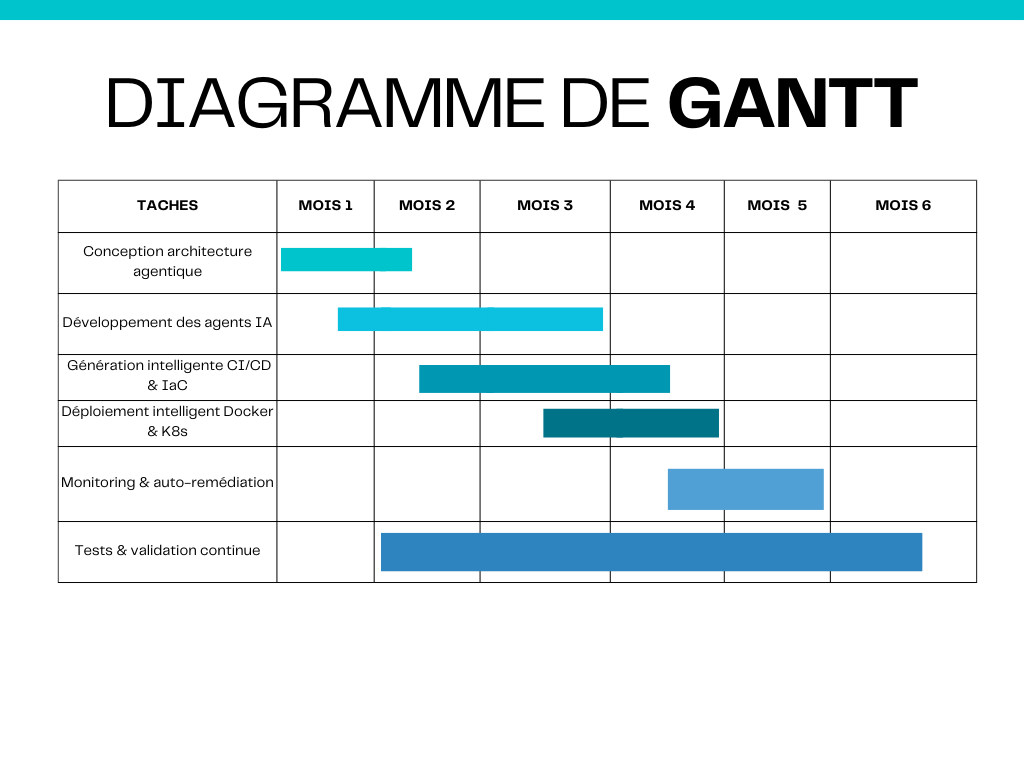
\includegraphics[width=0.95\textwidth]{images/Diag. GANTT.png}
    \caption{Planning du projet sur six mois (février $\rightarrow$ août 2026)}
    \label{fig:diagramme-gantt}
\end{figure}

\section{Conclusion}
Dans ce premier chapitre, nous avons présenté le cadre général du projet ainsi que
le contexte dans lequel il a été réalisé au sein de Talan Tunisie Consulting. Nous
avons exposé la problématique liée à la complexité des environnements Cloud et
DevSecOps modernes, ainsi que les limites des solutions existantes. Nous avons
ensuite décrit la solution proposée, puis la méthodologie Kanban adoptée pour la
gestion du projet. Le chapitre
suivant sera consacré à l'analyse et à la conception de la plateforme, en détaillant
l'architecture globale du système, les différents agents IA ainsi que les
technologies et mécanismes mis en \oe uvre pour la réalisation de la solution
proposée.
